\acresetall
\chapter{Introduction}
\label{chapter:introduction}

This dissertation develops an extensive analysis tool for the \ac{waas} to show that the statistical overbounding of \ac{ccc}, an integrity measure of \ac{waas}, can be reduced to increase availability without reducing integrity. The \ac{waas} is a navigational aid developed by the \ac{faa} with the goal of providing improved accuracy, integrity and availability of the \ac{gps}, giving aviation users the ability to use \ac{gps} in all phases of flight.  \ac{waas} augments standard \ac{gps} by providing regional range correction values associated with satellite ranging errors in GPS due to the ionosphere, which is the most significant contributor to environmental \ac{gps} ranging error.  \ac{waas} also provides corrections for any detected system errors from the system itself.  Standard \ac{gps} allows a user receiver (with an inaccurate clock) to estimate its range to multiple in-view satellites and, with ephemeris information to determine each satellite's position, \ac{gps} can compute an estimate of the user position as shown in Figure~\ref{fig:GPS-Basic-Overview}.

\begin{figure}
	\centering
	\scalebox{.5}{
	\mbox{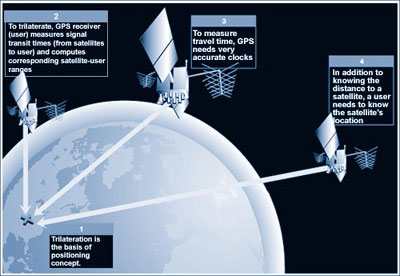
\includegraphics{figures/GPS-Basic-Overview.jpg}}
	}
	\caption{GPS Basic Overview. Translation is the basis of GPS positioning. A GPS receiver measures the signals transit times from satellites to the user and computes the corresponding satellite-user ranges. To measure travel time GPS needs a very accurate clocks. In addition to knowing the distance to the satellite, a user needs to know the satellites location.
  }
	\label{fig:GPS-Basic-Overview}
\end{figure}

\begin{figure}
	\centering
	\scalebox{.5}{
	\mbox{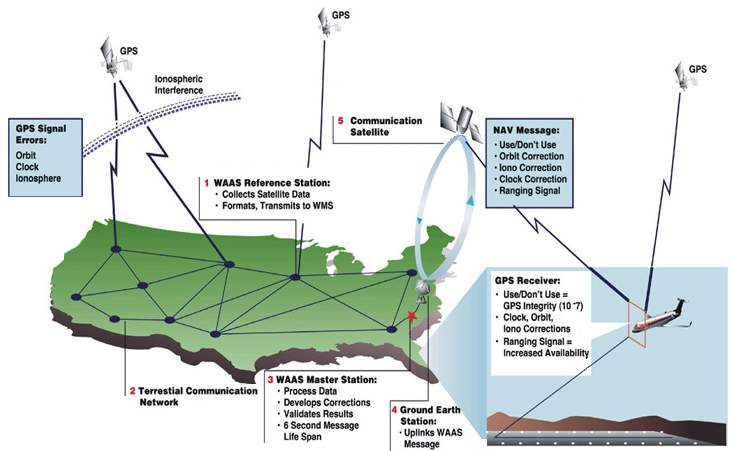
\includegraphics{figures/How-WAAS-Works.jpg}}
	}
	\caption{WAAS Basic Overview. The \acp{wrs} receive GPS measurements and transfer the data to the \ac{wms}. Integrity and differential corrections are generated and sent to the \ac{gus}.  The \ac{gus} trainsmits the \ac{wms} messages to a GEO Satellite which is broadcast down to users.
  }
	\label{fig:How-WAAS-Works}
\end{figure}

During normal operations, \ac{gps} \ac{sps} will have a user range error that is at or below a level required to support a positioning accuracy of 16 meters \ac{sep} \citep[p.51]{IS-GPS-200J}.  The \ac{waas} \ac{lpv} rquirement specifies Horizontal Accuracy  of $\leq 1.5m$ error 95\% of the time Vertical Accuracy $\leq 2m$ error 95\% of the time \citep[p.4]{WAAS-PAN-66} \citep[p.34]{FAA-E-2892b}. \ac{waas} routinely performs better than this [REFERENCE]. \ac{waas} estimates regional range correction values and provides these data to user receivers, which can incorporate the range corrections to improve the accuracy of the position solution, Figure~\ref{fig:How-WAAS-Works}. However, because the ranging errors are transmitted from a space-based component of the system, integrity checks must ensure that no false range corrections are transmitted that might cause significant erroneous position solutions.  There are a number of parameters in the \ac{waas} integrity checks that are statistically overbounded to ensure that no hazardous misleading information is transmitted to \ac{waas}-enabled \ac{gps} receivers.  Historically, the overbounding has been generous to provide significant safety tolerance [REF?], but no systematic study has been undertaken to identify which parameters are grossly overbounded and might possibly be reduced without affecting integrity. The purpose of this sensitivity analysis is to isolate the performance of the \ac{ccc} integrity monitor and show the gains made to reduce its bounding variance so that an increase in availability is attained while integrity is maintained. The purpose of the \ac{ccc} monitor is to detect satellite failures that cause the code phase and carrier phase of \ac{gps} to be incoherent.  Within \ac{waas} and the end-user equipment there is an assumption that the code and carrier are coherent, but there has never been an empirical analysis of its performance.  The complexity of the system, and the volume of data to be analyzed to provide reliable sensitivity results has never been addressed in the literature.
% If the code and carrier are assumed to be coherent, why do we need to monitor them?
% Don't we monitor them precisely because we know they might not always be coherent?
% I think this is better stated that the math requires the code and carrier to be coherent, so we monitor to ensure that this is the case.


% Make your first figure a basic GPS figure, then the WAAS system figure, then one that shows how corrections apply (see, for example, my Figure 2.7) Also, make your caption informative. It should have a title, then a description.  See any if my figures...
\begin{figure}
	\centering
	\scalebox{.35}{
	\mbox{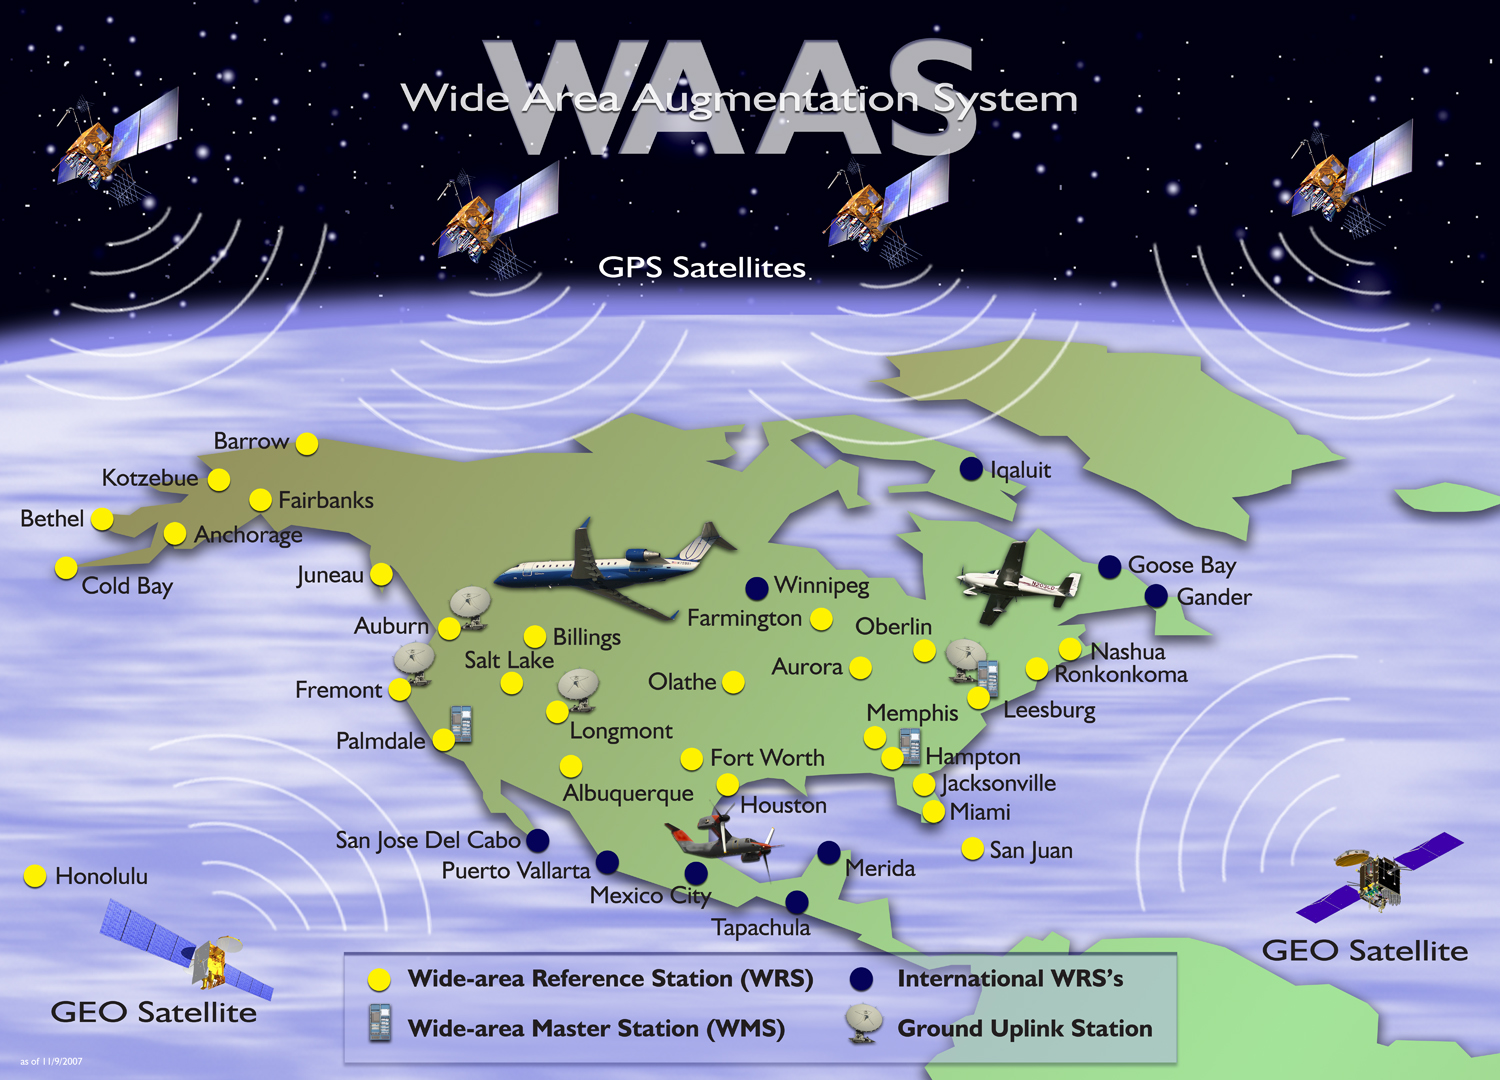
\includegraphics{figures/waas-overview-1.jpg}}
	}
	\caption{The Wide Area Augmentation System.  WAAS incorporates a number of reference stations in both the 48 contiguous United States as well as other North American partners: Mexico and Canada.  Three Master Stations calculate \ac{gps} satellite and ionosperic correction data and three GEO Satellites are use to transmit the information to aviation users.}
	\label{fig:WAAS-Overview-1}
\end{figure}


The stated goal of \ac{waas}, to provide improved accuracy, integrity and availability, is a complex set of tasks that may sometimes require tradeoffs between the competing goals.  The goals can be described as follows.  Accuracy is improved by providing a differential \ac{gps} solution, meaning \ac{waas} transmits range correction values for each satellite and the user \ac{gps} receiver applies these range correction values to the internally measured ranges prior to the user position computation.  This results in a \emph{differentially corrected} position solution that is more accurate than the position solution would be without the range corrections. The \ac{waas} architecture is a geographically diverse sensor network of high fidelity \ac{gps} receivers that track \ac{gps} satellites throughout North and Central America and Hawaii [FIG WAAS Overview here]. This network consists of 114 \ac{gps} receivers at 38 geographically diverse sites.  Each \emph{reference station} is precisely surveyed at the antenna phase center, so the range to any in-view satellite is known (assuming accurate ephemeris information allows for accurate satellite position computation. The \ac{gps} receivers in the reference stations use receive-time (of the transmitted satellite signal) to estimate satellite range, so any error in local receiver time translates directly into an error in the range measurement to the \ac{gps} satellite. To provide the highest degree of accuracy the \ac{gps} antennas are designed to mitigate multipath and each \ac{gps} receiver clock is disciplined with a cesium frequency standard to provide a highly accurate and precise time source [REF?]. A quarterly analysis of every second of every day is performed to observe if any change in the environment has occurred that may negatively affect performance. Yearly releases are conducted to update the antenna positions so that continental drift and other environmental factors are mitigated. The rigor put into this infrastructure enables this highly precise network of receivers to detect errors within \ac{gps} and the geographic diversity enables modeling of timing delays in the ionosphere. Once an end user within the \ac{waas} coverage area applies the \ac{gps} and ionospheric corrections sub-meter level \ac{gps} accuracy can be achieved in the best case and in the worst case range errors remain less than 2 meters. There are more than a dozen safety integrity monitors built into \ac{waas} that monitor \ac{gps} and ionospheric threats. Protecting users from integrity threats is an integral part of \ac{waas} as it was commissioned as a safety-of-life system, but integrity and availability have to be considered together as there is an inverse relationship between the two. As integrity increases availability is reduced. All \ac{gps} threats would be abated if \ac{gps} were not allowed to be used; integrity against \ac{gps} threats is 100\% while utilization of \ac{gps} is 0\%.  To achieve an acceptable level of utilization of \ac{gps} availability, confidence bounding is performed for \ac{gps} and ionospheric threats. The purpose of this study is to isolate the performance of the \ac{ccc} integrity monitor and show the gains made to reduce its bounding variance so that an increase in availability is attained while integrity is maintained. %You should note here that the tradeoff between availability and integrity is not strictly linear between 0 and 100.  You can increase availability from 0 to 95, and only reduce integrity in the nth decimal place.  10^-7, or something, right?, and use a REFERENCE!!!!!!!!

\ac{waas} has $\approx$2000 \ac{osp} values that define minimum and maximum limits, action thresholds, and timeouts [REF]. The parameters are used to control logic throughout the \ac{waas} system. There is always a balance between usability and safety.  For the \ac{faa} these two aspects are couched in the terms availability/continuity for usability and integrity for safety.  If the system remains off then this is the highest level of integrity, meaning if the user does not use the \ac{gps} then they are safe against all \ac{gps} related threats.  This would not make a practical system, so it led the engineers developing the \ac{waas} application to use values that would allow the system to be usable, but were significantly conservative to protect the user against \ac{gps} related threats.  At the inception of \ac{waas} there was insufficient empirical data to appropriately set many of the integrity bounding limits.  At least one value was stated as being grossly overbounded and that the empirical evidence to set it correctly would require many years of data [REF for which value you are talking about].  The \ac{nase} organization has now accumulated several years of data, but there is currently no analytical system in place to process this volume of data so that updated \ac{osp} values can be set.

A sensitivity analysis of the type proposed in this study is difficult due to the shear magnitude of data to be analyzed. In order to properly analyze the sensitivity of \ac{waas} to the level of statistical overbounding of the \ac{ccc} parameter, many years of data must be analyzed.  This ensures that seasonal effects, a broad selection of significant weather events, and any astronomic effects can be included in the analysis [REF about what external things might affect integrity].  However, the system requirements for just the hardware and software present a significant barrier to achievement. Not only is significant processing power required, but an effective data handling method must also be employed so that the results are discoverable from the plethora of numerical information generated.  %Can you find a CS reference about such a system and its complexity?

%The cost of establishing and maintaining a high fidelity \ac{gps} monitoring network is considerable. Establishing the infrastructure and algorithms for the \ac{ioc} of \ac{waas} cost the United States government over \$4 Billion and the yearly maintenance cost are approximately \$100 million per year. Costs of this level prohibit all but a few countries from establishing a monitoring system of this magnitude. Further attaining access to the data along with the infrastructure to store and analyze the data is cost prohibitive. Over my tenure at the \ac{faa} there has been a concerted effort to establish the capability to perform an analysis of this extent. The infrastructure for collecting, storing and analyzing data at this volume has cost over \$5 million to establish and has pushed the limits of hardware and software.

The cost of establishing and maintaining the infrastructure for \ac{waas} is significant.  In addition to the 3 geosynchronous satellites keeping station above North America, there are the 38 reference station sites, three master reference stations, and six uplink stations, as well as the infrastructure to record and analyze daily information for uplink to the satellites.  Indeed, $\approx$374,284,800 data points are generated every day for analysis.  A major obstacle to performing any sensitivity analysis of the various overbounding parameters lies in the sheer volume of data that must be processed.  It should be noted that in order to glean any meaningful results, extended periods of historical raw data must be processed to ensure that seasonal variations, weather events, and astronomical transients (solar flares, magnetic storms, etc) are included in the analysis.  This research incorporates a system that is novel in itself.  The system capable of the desired analysis has taken several years and significant funding to develop. The system approach in this study utilizes commodity hardware and open source databases, programming languages and analytics software, with the goal of processing seven (7) years of data to assess the sensitivity of \ac{waas} to the \ac{ccc} parameter.  However, the system has been designed with the concept of scalability at the forefront, so that it can be expanded to assess other system sensitivities in the future.

%Though there was considerable time, effort and funding in establishing the capability outlined in this study, the approach in this study utilizes commodity hardware and open source databases, programming languages and analytics software. Further this capability was established to analyze as very specific data set. For the range measurements alone there are $\approx$374,284,800 data points per day.  The equipment required to process this was scaled commensurately for the data that is collected each day times the 7 years of data collected. Over 950 billion data points for just a single type of measurement and several hundred data elements are stored. The approach utilized in this study can be scaled appropriately to the application domain so cost for establishing a similar capability is tenable.

The approach outlined in this analysis is innovative in that it can be utilized to increase the availability of any Space Based Augmentation System while maintaining integrity.  This infrastructure is limited to all but a few countries, but with the countries that are developing this capability, world wide space based augmentation can be attained. The application of this methodology could lead to the establishment of highly available space based navigational aids on a global level. Further. the generalized approach utilized to solve this big data analytics problems can be utilized in domains outside of this specific aviation application.

Global SBAS Picture

\href{https://www.gps.gov/policy/funding/2017/}{https://www.gps.gov/policy/funding/2017/}

\href{http://commdocs.house.gov/committees/Trans/hpw106-100.000/hpw106-100\_1.HTM}{http://commdocs.house.gov/committees/Trans/hpw106-100.000/hpw106-100\_1.HTM}

\href{https://www.gps.gov/technical/ps/2008-waas-performance-standard.pdf}{https://www.gps.gov/technical/ps/2008-waas-performance-standard.pdf}

Things I need.

PRN SVN Mapping for the last five years.
Assign to Hoang.


First sentence what this dissertation has achieved.
30,000ft view of \ac{waas} and the Problem. Pros and Cons of \ac{waas} and the specific area I am looking at.

Paragraph 1: What is the problem?

Not more than 3-4 sentences telling the reader what the problem is, in as simple English as possible

Paragraph 2: Why is the problem hard?

What has eluded us in solving it? What does the literature say about this problem? What are the obstacles/challenges? Why is it non-trivial?

Paragraph 3: What is your approach/result to solving this problem?

How come you solved it? Think of this as your “startling” or “sit up and take notice” claims that your dissertation will plan to prove/demonstrate

Paragraph 4: What is the consequence of your approach?

So, now that you’ve made me sit up and take notice, what is the impact? What does your approach/result enable?
~\\

%This paragraph belongs above...I attempted to put it where it seems to fit...%


%Don't need any of this next paragraph in the Intro%
%Currently in this research effort the beginnings of a system have been created that can be used as an analytics platform for getting the varying data formats and elements into a common format where meaningful analysis can be performed.  Every component in the system is purposely selected or designed to take data from its rawest form and process it into a format that can be utilized, manipulated and assessed. As of this writing the system can process NovAtel GUST, G-II and G-III \ac{gps} receiver binary log files. The software can identify receiver log messages, \ac{crc} check that the messages is valid and break each message type into its constituent elements for storing and further analysis. This has been fully demonstrated end to end on a \ac{geo} Satellite monitoring system in development. This system is currently monitoring one \ac{geo} satellite at one \ac{gus} site but will be expanded to four \ac{geo}s at 8 \ac{gus} sites in the near future. It process data from the \ac{waas} application receiver and a second receiver used for fault isolation. The system is logging $\approx$1213 data elements per second from only two message types and this number will grow as more message types are recorded to the database.
